
\subsection{The Easy Method}
\label{easyinstall}\index{RTXI, Live CD, Live USB, installation, easy install}

The Live USB provides a complete real-time Linux operating system with RTXI without installing anything on your computer. Within the live environment, you can mount your hard drive and technically run experiments, though real-time performance will be slower compared to that of an actually installed system. For actual experiments, we strongly recommend installing RTXI and the entire operating system environment on your hard drive. This can be easily done from within the Live USB. 

\textit{Note:} You do not need a DAQ card installed to test the Live CD or for RTXI to run.

The Live USB is distributed as an ISO image on our website (www.rtxi.org) for both 32 and 64-bit systems. To decrease the size of the Live USB, we removed many  common desktop applications, such as LibreOffice, that can easily be reinstalled later. Note that while the image can be burned to a DVD and then run, there will be significant speed limitations. 

To install the live image to a USB, follow these steps:

\begin{enumerate}
\item \textbf{Download the image.} Pick the one that corresponds to your processor's architecture. As a general rule, systems built in the past few years support 64-bit, but if your machine is old, try the 32-bit one. 

\item \textbf{Download Unetbootin.} (http://unetbootin.sourceforge.net/) Unetbootin is a cross-platform (Windows, Linux, and OS-X) application that can install a bootable .iso image to a USB. When it starts, you will see a window similar to this:

\begin{figure}[h]
\begin{center}
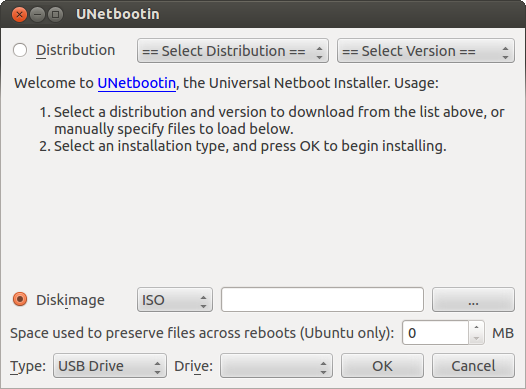
\includegraphics[width=4.5in]{unetbootin-open.png}
\caption[Unetbootin]{Unetbootin is a cross-platform program that burns ISO images to bootable media.}
\end{center}
\end{figure}

\item \textbf{Format a flash drive.} Format your USB drive to FAT32. Note that this process will wipe all the data already on the drive. If you do not know how to do this, Unetbootin should be able to do it for you. 

\item \textbf{Burn the ISO.} Select the second option to pick the ISO file you want to burn. In the dialog window that opens, select the image you downloaded in step 1. Then, select the USB where you want to install RTXI. If you are using Ubuntu, you may want to use the persistence feature available as ``Space used to preserve...". This allows you to add/modify files and have the changes saved from one session to another. Without it, all changes to the live environment are lost when the system shuts down.

\textit{Note of caution:} Be sure you know which drive is which. If you accidentally write to the wrong drive, you will lose any data already stored on it. 

Once everything is set, click ``OK" to start the installation process. 

\item \textbf{Boot using the Live USB.} Once the Unetbootin is finished, shut off your system. By default, your computer may not be configured to boot off a USB drive. When you turn on your computer, you will have to press ``F2", ``F4", or another F key depending on your computer to access your BIOS menu. The following instructions use the BIOS of our system, but your will likely be similar. 

\begin{figure}[h]
\begin{center}
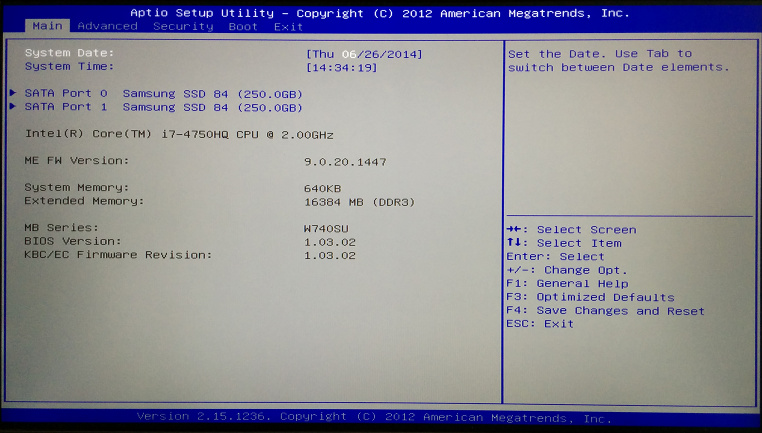
\includegraphics[width=4.5in]{bios-1v2.jpg}
\caption[BIOS page]{The BIOS provides low-level control over system functions, such as the media used to boot an operating system.}
\end{center}
\end{figure}

You can navigate though the menu using the arrow keys of your keyboard. Press ``Enter" to select a highlighted option and ``Esc" to move from a sub-menu to its parent menu. Navigate to ``Boot" or some similar window and change the boot order. 

\begin{figure}[h]
\begin{center}
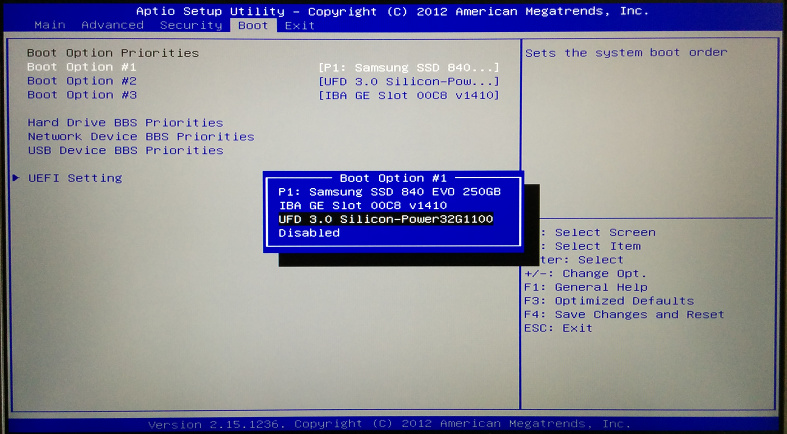
\includegraphics[width=4.5in]{bios-2v2.jpg}
\caption[BIOS boot order]{The ``Boot" tab provides options to change the boot priority of different media.}
\end{center}
\end{figure}

Move to EXIT, save the changes, and exit BIOS. 

\begin{figure}[h]
\begin{center}
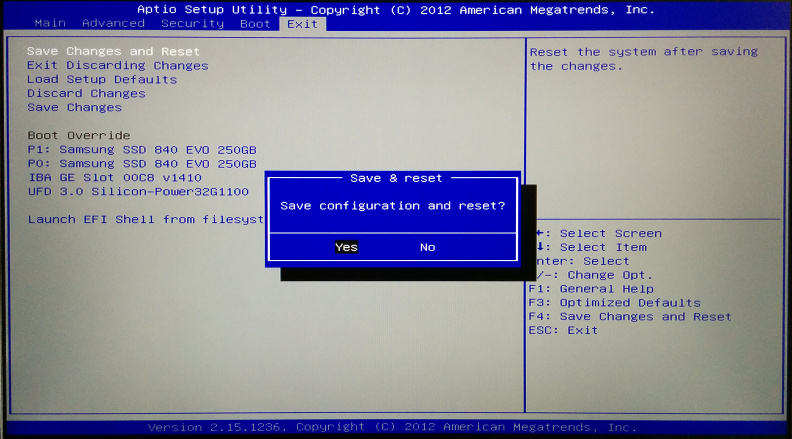
\includegraphics[width=4.5in]{bios-3v2.jpg}
\caption[BIOS exit]{To implement changes, save them and then restart the system. At this point, any changes to boot media priority will be applied.}
\end{center}
\end{figure}

Your system will restart and should now boot into your Live USB. In some cases, Ubuntu will correctly load but will drop you to a shell prompt rather than the GUI. This is usually due to video drivers that were not bundled directly into the kernel or were not able to be loaded. If you see a shell prompt, try starting the GUI by typing:

\begin{example}
\# startx
\end{example}
\end{enumerate}

To install RTXI from the live environment to your hard drive, follow these steps. 

\begin{enumerate}
\item \textbf{Start the installation program.} To start, double-click the ``Install" icon on the desktop.

\item \textbf{Set configuration options.} Answer all the setup questions. If you are in the U.S., the default choices will likely suffice. 

\item \textbf{Choose a partitioning scheme.} The installer provides several options for installing Linux on a hard drive. You can:
	\begin{enumerate}
	\item \textbf{Erase the hard drive and install the operating system.} To do this simply choose ``Erase hard drive and install". Remember, once the hard drive is erased, all previously stored information will be lost, so make sure to select the correct drive and check that no needed files have been left on it. 
	\item \textbf{Install the operating system alongside an existing one(s).} This option is called dual-booting, where two or more operating systems are present. Users are prompted at boot to select which one to use. 
	\end{enumerate}

For users who want to dual-boot Ubuntu with another operating system, below is an example of a computer with two hard drives, each of which has a single partition defined. 

SATA hard drives are listed as sdX where X is either a letter or a number. In our case, \texttt{sda} refers to the first hard drive connected to the motherboard (in this case the SATA0 slot) and \texttt{sdb} is the second hard drive. If you have IDE rather than SATA hard drives, you should see \texttt{hda} drive designations. 

\begin{figure}[h]
\begin{center}
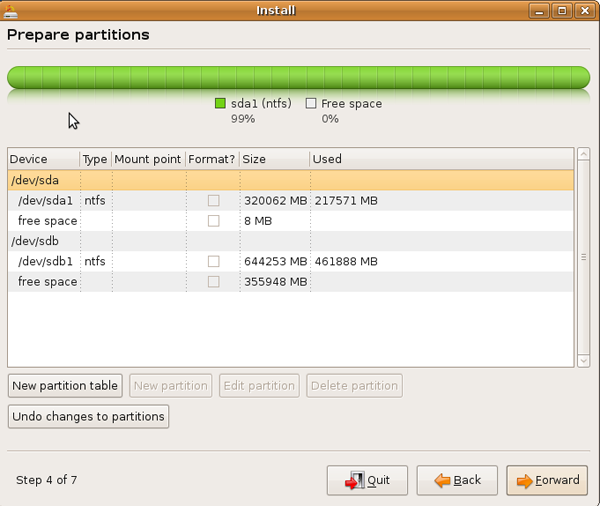
\includegraphics[width=4.5in]{livecd1.png} 
\caption[Ubuntu Installation: Preparing your partitions]{The Ubuntu installer allows you to reconfigure your partitions. This configuration shows a single Windows partition (\texttt{/dev/sdb1}) in NTFS file format that uses the entire second hard drive (\texttt{/dev/sdb}).} 
\end{center}
\end{figure}

\texttt{sda1} is the first and only partition on the first hard drive. The second hard drive has about 35GB of free space in which to create new partitions for Linux. If you don't have any free space for Linux, you will need to resize your partition. Do this by clicking on it (eg. \texttt{/dev/sdb1}) and then on ``Edit Partition." You will get a pop-up window with a colored bar representing the partition. Use your mouse to drag the right edge of the colored bar so that the partition is smaller, leaving you with unallocated free space at the end. Hit ``OK" and you should see that on \texttt{/dev/sdb} you have a \texttt{/dev/sdab} partition and more free space.

\item \textbf{Set up a SWAP partition.} Linux uses a special partition called SWAP to augment RAM and increase the total amount of virtual memory available to running applications. This allows Linux to move unused files from RAM to SWAP, freeing up fast-operating RAM for new processes, and it avoids problems arising from running out of RAM, which causes the Linux scheduler to random kill processes to free memory.  Note that SWAP exists on the hard drive and doesn't not perform nearly as quickly as RAM. Systems that have to access SWAP frequently will have significantly degraded performance. 

For RTXI, SWAP is needed mainly for avoiding process-killing behavior. If you have 3 or more GB of RAM, 1-2GB of SWAP will suffice. If you only have 1-2GB of RAM, you should add 2GB of swap space. You should also consider adding more RAM. Using SWAP will degrade real-time performance. To add SWAP, from within the installer, click on the free space in your partition table and click ``New Partition." The default size of a new partition is the rest of the free space on the hard drive so decrease it to the desired size of your swap partition and select the type as ``swap."

\item \textbf{Set up the Linux partition.} For the actual Linux OS, make another new partition in the remaining free space. This one should be a ``Primary" partition and set the mount point to be a single forward-slash ``/". Set filesystem format as ext4. 

You may also want to leave some extra room for a data partition that is read/write-able in both Windows and Linux. This partition should be formatted as NTFS. Note that FAT32 can only handle file sizes up to 4GB. You can have up to 4 primary partitions. If you need more, you need to create an extended partition under which you can create as many ``logical" partitions as you like.

\begin{figure}[h]
\begin{center}
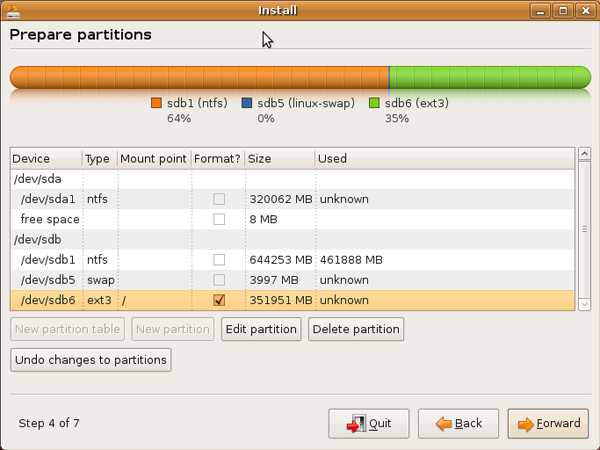
\includegraphics[width=4.5in]{livecd2.png} 
\caption[Ubuntu Installation: Dual booting Window and Linux]{This configuration shows a hard drive (\texttt{/dev/sdb}) partitioned to dual boot Windows and Linux. The Windows NTFS formatted partition remains and was simply resized. There are additional Linux swap and Linux ext4 formatted partitions as well. The ext4 partition is set to the root \texttt{/} mount point and has been selected to be formatted. The NTFS partition is NOT going to be formatted so no data will be lost.} \end{center}
\end{figure}

\item \textbf{Linux installation.} Your new Linux partition should have a flag indicating that the hard drive space will be formatted. If you are dual-booting, make sure your Windows (NTFS) partition is NOT set to be formatted if you want to keep your data. When you're all done setting up your partitions, click ``Forward." You can always restart the hard drive partitioner in Linux to resize your partitions. If you decide you need more room in Linux, you can cancel your changes and repeat the previous two steps, this time shrinking down your existing OS even more. 

When satisfied with your settings, start the installation. 

\item \textbf{Boot into the GRUB menu.}In addition to the OS, the installer will set up a program called GRUB. When you reboot your computer, GRUB will set up a menu that where you choose which OS to boot. Note that if you ever re-install Windows, GRUB will get overwritten, and the OS-selection menu will no longer appear. Linux will still exist on your hard drive. You will just need to reinstall GRUB using a Live CD.

\item \textbf{Start RTXI.} Now, with our Linux OS installed, you can start RTXI. From the terminal (CTRL+ALT+T), enter:
\begin{example}
\$ sudo rtxi
\end{example}

You will be prompted for the password you set up when you installed Ubuntu and logged in to your system. Enter this, and RTXI will start. 

\end{enumerate}